
\title{Recap Computer Architectures (02LSEOV)}
\author{Jacopo Nasi\\
        Computer Engineer\\
        Politecnico di Torino}
\date{I Period - 2017/2018\\\bigskip\bigskip\today}

\documentclass[12pt]{article}
\usepackage[utf8]{inputenc}
\usepackage[italian]{babel}
\usepackage{geometry}
\usepackage{indentfirst} % First line indent
\usepackage{mathtools}
\usepackage{wrapfig}
\usepackage[usenames, dvipsnames]{color}
\usepackage{float}
\usepackage{amssymb}
\usepackage{ifsym}
\usepackage{listings}
\usepackage{multicol}

% Misure Documento
\geometry{ a4paper, total={170mm,257mm},left=35mm, right=35mm, top=35mm, bottom=35mm }

\begin{document}

\begin{figure}
  \centering
  
\includegraphics[width=10cm]{images/polito.pdf}
\end{figure}

\maketitle

\newpage
\tableofcontents

\newpage
{\noindent \Large \textbf{License}\bigskip}

This work is licensed under a Creative Commons Attribution-NonCommercial-ShareAlike 3.0 Unported License.\\
You are free:
\begin{itemize}
  \item \textbf{to Share}: to copy, distribute and transmit the work
  \item \textbf{to Remix}: to adapt the work
\end{itemize}
Under the following conditions:
\begin{itemize}
  \item \textbf{Attribution}: you must attribute the work in the manner specified by the author or licensor (but not in any way that suggests that they endorse you or your use of the work)
  \item \textbf{Noncommercial}: you may not use this work for commercial purposes.
  \item \textbf{Share Alike}: if you alter, transform, or build upon this work, you may distribute the resulting work only under the same or similar license to this one.
\end{itemize}

\noindent More information on the Creative Commons website (http://creativecommons.org).

\begin{figure}[h!]
  \centering
  
\includegraphics[width=3cm]{images/license.png}
\end{figure}

{\noindent \Large \textbf{Acknowledgments}\bigskip}

Questo breve riepilogo non ha alcuno scopo se non quello di agevolare lo studio di me stesso, se vi fosse di aiuto siete liberi di usarlo.\\
Le fonti su cui mi sono basato sono quelle relative al corso offerto (\textbf{Computer Architectures (02LSEOV)}) dal Politecnico di Torino durante l'anno accademico 2017/2018.\\
Non mi assumo nessuna responsabilità in merito ad errori o qualsiasi altra cosa. Fatene buon uso!
\newpage

\section{Introduction Computer Design}
\subsection{Computer Evolution}
The first general-purpose computer was created in the late 40s. What now we can buy for 500\$ is equivalent (performance) to what could be bought for about \$1M in 85'.\\
During the years the performance growth was not linear, as you can see in figure \ref{fig:cpugrowth}, during the first 10 years the annual increase was around 25-30\%/year, from the late 80s to the 2000 the growth is increased around 50\%/year and, in the last few years it decrease to the 22\%. Why this change during the increase?\\
\begin{figure}[h!]
  \centering
  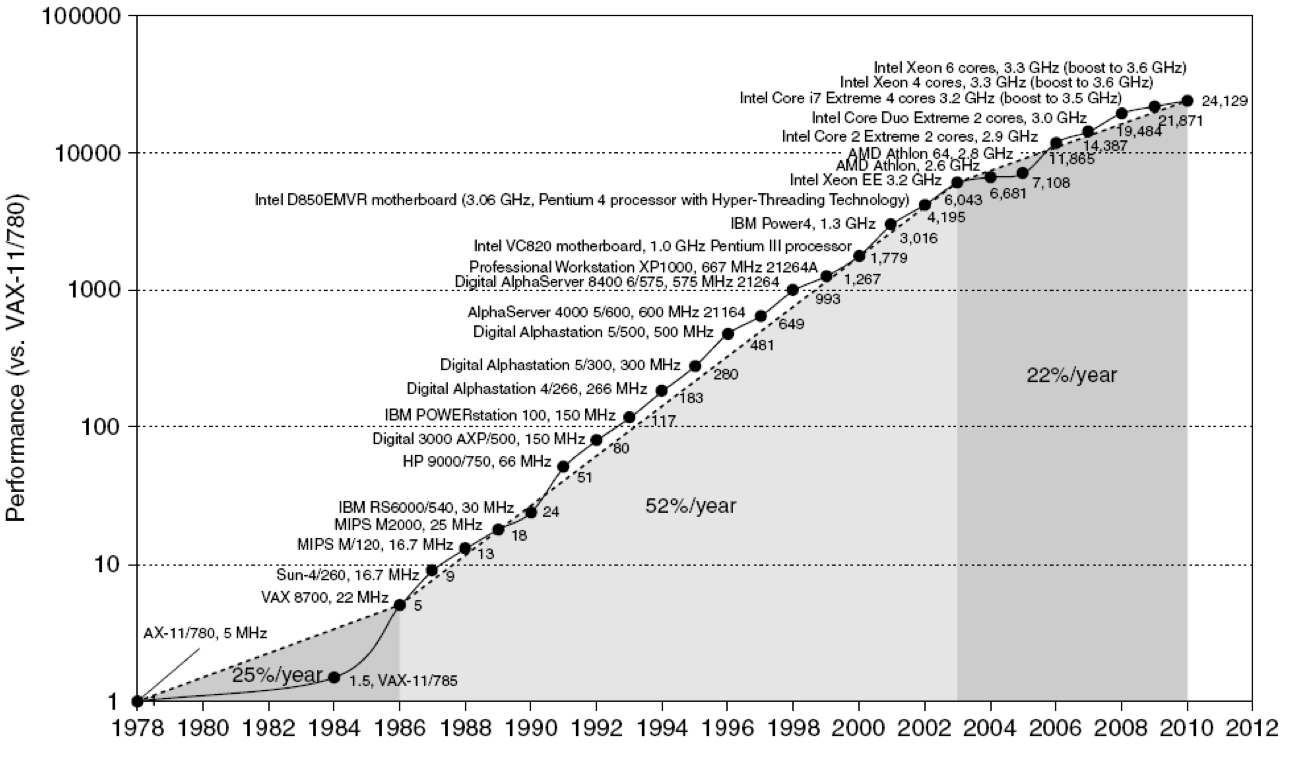
\includegraphics[width=\linewidth]{images/cpugrowth.png}
  \caption{CPUs Growth over years}
  \label{fig:cpugrowth}
\end{figure}
The manufacturers have found a lot of physical problem related to the creation of new products, this problem are mainly related to:
\begin{itemize}
  \item Power-Issue.
  \item Lower instruction-level parallelism.
  \item Unchanged memory lantecy.
\end{itemize}
in fact, since 2004, the major industry have changed the conceptual ways to desing processors, switching from single to multi-core architectures. We can say that, in anytime, this growth is incredible an is due to improvements in technology, microprocessor architecture and software development. Since the multi core introduction the major prefers to investe on multicore system rather than develop faster CPU.\\

\subsection{Designing}
There are 5 main market areas:
\begin{itemize}
  \item \textbf{Personal Mobile Device} (PMD): Smarthphone, tablet. They are focused in energy efficency and real-time app.
  \item \textbf{Desktop Computing}: From PC to workstation and the main pourpose is optimize the price-performance ratio.
  \item \textbf{Server}: Larger-scale and more reliable computing services.
  \item \textbf{Cluster - WAS}:Emphasis on availability, price-performance and power consumption.
  \item \textbf{Embedded Computers}: Fastest growing portion of PCs market. All special-purpose computer-based application, from cheap to high-end processors.
\end{itemize}
There are to \textbf{Classes of Parallelism}:
\begin{itemize}
  \item \textbf{Data-Level} (DLP): Many data items that can be operated on at the same.
  \item \textbf{Task-Level} (TaskLP): Many task of a work can operate independently.
\end{itemize}
The first solution allow the processor to split the data operation over multiple cores, you can for example divide an array of n elements over 4 core and, if T is the computational time needed for the entire array, the final time will be T/4 plus a little time for the reunion of the data. It split the one task on different data.\\
The TLP instead is able to manage multiple task over the same data, this is the common behavior of the actual system (pipelining techniques).\\
There are different Parallel Architectures:
\begin{itemize}
  \item \textbf{Instruction-level} (ILP): The is modestly use the data-level parallelism.
  \item \textbf{Vector and GPU}: It exploits DLP.
  \item \textbf{Thread-level} (TLP): It exploits DLP and TaskLP.
  \item \textbf{Request-level} (RLP): Exploits parallelism among decoupled (not-related) tasks.
\end{itemize}
The designing of a new computer involve important analysis to the main pourpose of it, you need to study which attributes are important for the new machine and you need to maximizes performance and matching cost and power constraints. During the last decade the PC design took advantage of architectural and technology improvements, the performance increase is more than a factor of 15 on what would have been obtained by relying solely on technology.\\

The \textbf{Moore's Law} says that: \textit{The number of transistors that can be integrated into a single chip doubles every 18/24 months}. Until now the law has worked, as you can see in the figure \ref{fig:moore} and, probably, it will work for other time.

\begin{figure}[h!]
  \centering
  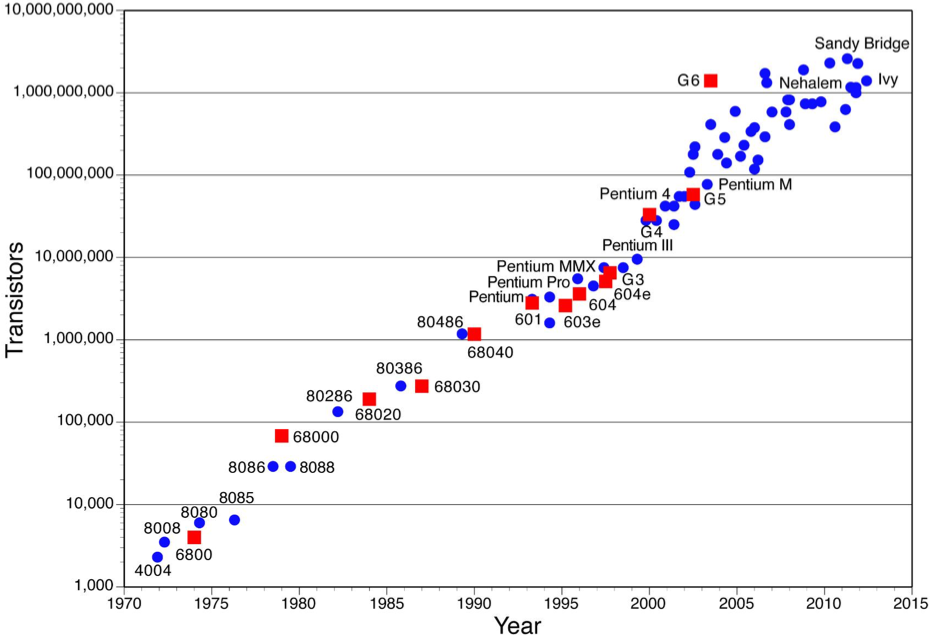
\includegraphics[width=\linewidth]{images/moore.png}
  \caption{Transistors growth on CPUs}
  \label{fig:moore}
\end{figure}

\paragraph{Cost} During the evaluation of the IC manufacturing cost it is important not to forget the impact of yeild, the percentage of products that pass the test phase. The production process for every product undergoes an evolution which normally leads to an improvement in yield (learning curve). The cost decrease is due to yield increase. Probably the most important part of the manufacturing cost is related to the validation and testing procedures.\\

\paragraph{Other designing problem} The continuos increase of the system complexity and device integration leads to porblem with power consumption, for the Power and for the Energy (manly for portable devices). Until now the greater power consumption contribution is due to the trasnsistor switching phase, related to the physical formulas the solution applied is trying to reduce the voltage.\\
Another important factor is the \textbf{Dependability} that is the quality of the system to deliver a correct service, is traditionally very high, but it can be lowered by software or hardware bugs both during the production or in designing phase. During this years the safety-critical areas where the microprocessor have relevant importance are increased, initialy only space, avionics and nuclear, but now we have rail-road, automotive, biomedical, telecom, ecc...\\
The dependability is often measured using:
\begin{itemize}
  \item \textbf{Mean Time To Failure} (MTTF): 1 failure in one billion hours.
  \item \textbf{Mean Time Between Failures} (MTBF)
  \item \textbf{Mean Time To Repair} (MTTR)
\end{itemize}
This three measures are related by the formula: $MTBF = MTTF + MTTR$

\paragraph{Performance} they be analyzed under multiple point of view, \textit{Time between start and completion of an operation, Total amount of work done in time unit, ecc...}. The UNIX system provide 4 different values:
\begin{itemize}
  \item Elapsed time
  \item CPU Time
  \begin{itemize}
    \item User
    \item System
  \end{itemize}
\end{itemize}
The evaluation of often performed letting work a computer and observing its behavior. Unfortunately, the choice of the application severely affects the performance and is not too easy looking the result in a correct way. The main solution is using benchmarks to compare different system running the same operation and production comparable times of execution. The benchmark sets are normally composed of:
\begin{itemize}
  \item Kernels
  \item Program Fragments
  \item Applications
\end{itemize}

There are multiples solution to analyze the performance one of the most common is the \textbf{Amdahl's law} and it based to the comparisons with the older version of the same product. The speedup is calculated by this formula:
\begin{equation}
  \begin{gathered}
    Speedup = \frac{Performance_{enhancement}}{Performance_{NOenhancement}}
    \label{eq:tsoglie}
  \end{gathered}
\end{equation}
the value depends on two factors:
\begin{itemize}
  \item $Fraction_{Enhanced}$: the fraction of the computation time that take advantages of the enhancement.
  \item $Speedup_{Enhanced}$: the suze of the enhancement on the part it affects.
\end{itemize}
A more complete formula is:
\begin{equation}
  \begin{gathered}
    Speedup_{overall} = \frac{1}{(1-Fraction_{Enhanced}) + \frac{Fraction_{Enhanced}}{Speedup_{Enhanced}}}
    \label{eq:tsoglie}
  \end{gathered}
\end{equation}
an example could be useful:\\

\textit{An enhancement makes one machine 10 times faster for 40\% of the programs the machine runs. Which is the overall speedup?}\\
Fraction = 0.4, Speedup = 10.
\begin{equation}
  \begin{gathered}
    Speedup_{overall} = \frac{1}{(1-0.4) + \frac{0.4}{10}} = 1.56
    \label{eq:tsoglie}
  \end{gathered}
\end{equation}

Another important designing evaluation is measuring the time required to execute a program, the are severals approaches:
\begin{itemize}
  \item Observing the real system: Not easy to be evaluated.
  \item Simulation: It could be really expensive.
  \item CPU Equation.
\end{itemize}
the latest solution use a provided formula to evaluate the CPU time:
\begin{equation}
  \begin{gathered}
    CPU_{Time} = CLK_{Time}*\sum_{i=1}^n{CPI_{i}*IC_{i}}
    \label{eq:tsoglie}
  \end{gathered}
\end{equation}
where:
\begin{itemize}
  \item \textbf{$CPI_{i}$}: Number of clock cycles required by instruction i (depends on hardware and instr set).
  \item \textbf{$IC_{i}$}: Number of times instruction i is executed in the program (depends instruction set and compiler).
  \item \textbf{$CLK_{Time}$}: Inverse of clock frequency (depends technology).
\end{itemize}
in the pipelined processor, $CPI_{i}$ may vary for a given instruction, therefore the evaluation becomes much harder.
% END Part 1 - Introduction

\section{Instruction Set Principles}
\subsection{Introduction}
The Instruction Set Architecture (ISA) is hoe the computer is seen by the programmer or the compiler. There are different kind of design and they can be selected by different characteristics. The CPUs are often classified according to the type of their internal storage:
\begin{itemize}
  \item Stack: Is the simplest one it can't accessing memory during operations.
  \item Accumlator: Similar to 8051 can access the memory during operation.
  \item Registers
  \begin{itemize}
    \item Register-memory: Similar to 8086, have a 16-bit register.
    \item Register-Register (load-store)
    \item Memory-memory (no real cases)
  \end{itemize}
\end{itemize}
Nowadays all processors are General-Purpose Register (GPR) this because registers are faster than memoery and are easier for a compiler to use. The CPUs are also classifiable by the number of operant per ALU instruction (2 or 3) and number of memory operand per ALU.\\

\subsection{Memory}
The memory has a fundamental work in the CPU world, there are several different type of it and of course different type to how accessing it.\\
There are many different \textbf{memory addresses} that can be implemented:
\begin{itemize}
  \item \textbf{Little Endian}: Byte with lower address at the least significant position. The addresses of the data is that of the LSB.
  \item \textbf{Big Endian}: Byte with lower address at the most significant position. The addess of the data is that of the MSB.
  \item \textbf{Aligned}: Allowing only aligned accesses to memory could is a limitation in terms of performance.
  \item \textbf{Misaligned}: This solution require hardware and performance overhead.
\end{itemize}
A memory position can be accessed in different ways:
\begin{itemize}
  \item \textbf{Register}: (ADD R4, R3) when a value is in a register.
  \item \textbf{Immediate}: (ADD R4, \#3) for constants.
  \item \textbf{Displacement}: (ADD R4, 100(R1)) accessing local variables.
  \item \textbf{Deferred or Indirect}: (ADD R4, (R1)) accessing using a pointer or a computed address.
  \item \textbf{Indexed}: (ADD R3, (R1 + R2)) useful in array addressing: R1=array base, R2=index.
  \item \textbf{Direct or Absolute}: (ADD R1, (1001)) useful for accessing static data.
  \item \textbf{Indirect}: (ADD R1, @(R3)) if R3 is the addr. of a pointer p, then the mode is like \*p.
  \item \textbf{Autoincrement or decrement}: (ADD R1, (R2)$\pm$) useful for stepping through array within a loop.
\end{itemize}
Is important to choosing the correct addressing mode, one can obtain some important consequences, from reduing the number of instruction to increasing the architecture.\\
There are a lot of instruction that can be done, looking at the 80x86 frequency we can see that most most used are \textit{Load, Conditional Branch, Compare and Store} that are around the 70\% of the total operation performed.\\
The instruction set encoding depends on which instruction compose the instruction set and which addressing modes are supported. When a high number of addressing modes is supported, and address specifier is used to specified the addressing mode. When the number of addressing modes is low, they can be encoded together with the opcode. The different encoding are:
\begin{itemize}
  \item \textbf{Variable}: Any number of operands, operation with variable length, lower performance and minimum code size.
  \item \textbf{Fixed}: Fixed number of operands, need address specifier, fixed instruction length, maximum performance but larger code size.
  \item \textbf{Hybrid}: Multiple format specified by the opcode and it allows a trading-off between code size and performance.
\end{itemize}

Assembly-level programs are now produced by compilers only. The CPU designer and the compiler writer must interact and cooperate. A crucial part taken by the compiler is the optimization of the register using, it easier to solve it when the number of register is higher ($>$16).

\section{Pipelining}
\subsection{Introduction}
Pipelining is an a solution to execute multiple instructions at the same time overlapping it. The different units (also called \textit{stage} or \textit{segment}) are completing different part of different instruction in parallel. The figure \ref{fig:pipe_ex} is an example of this techniques.
\begin{figure}[h!]
  \centering
  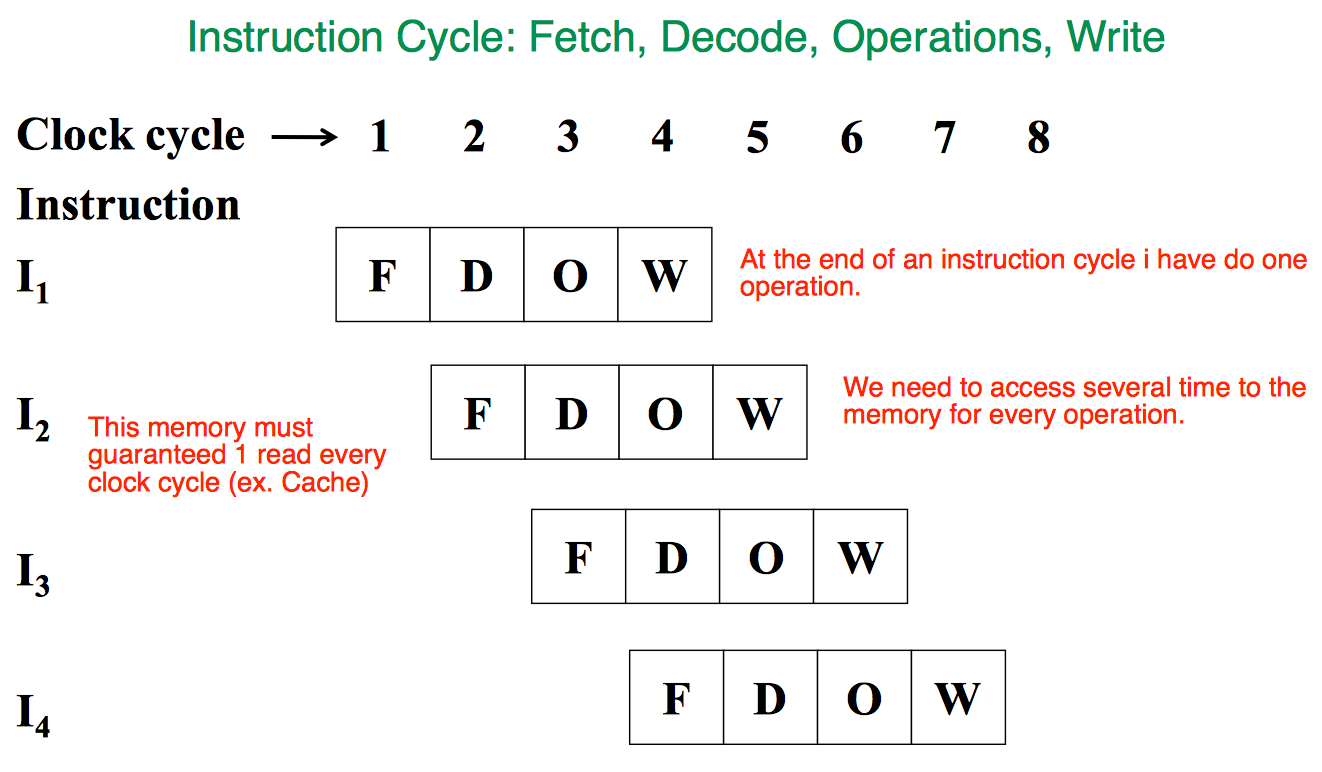
\includegraphics[width=\linewidth]{images/pipe_ex.png}
  \caption{Pipeling example}
  \label{fig:pipe_ex}
\end{figure}
The \textbf{throughput} of a pipelined processor is the number of instructions which exit the pipeline in the time unit. All the pipeline stages are synchronized (they proceed to executing the new task all together); the necessary time for executing one step is called machine cycle and, normally, corresponds to one clock cycle. Of course the duration of a machine cycle is determined by the slowest stage. CPI means clock cycles per instruction. The ideal pipeline have all stages perfectly balanced, in this way the $TRP_{pipelined} = TRP_{unpipelined} * n$ where \textit{n} is the number of pipeline stages.

\subsection{behavior}
The execution of each instruction may be composed of at most five clock cycles:
\begin{itemize}
  \item \textbf{IF}: Fetch the instruction from the memory address of the PC and save it in the IR.
  \item \textbf{ID}: Decode the instruction just fetched.
  \item \textbf{EX}: Execute the instruction.
  \item \textbf{MEM}: Memory access and brach completion.
  \item \textbf{WB}: Write-back.
\end{itemize}
with the unpipelined processor all instruction require 5 CC, the only optimization to reduce the average CPI is completing the ALU instruction during the MEM cycle, hardware resources could be optimized avoiding duplications.\\
The pipelined version instead can be more powerful beacause a new instrcution is started at each clock cycle and different  resources work on different instruction at the same time. There are several consideration to keep in mind during the development of this units; at every clock cycle, each resource can be used for one purpose only, this means that:
\begin{itemize}
  \item Separate instruction and data memories must be used.
  \item The register file is used in two stages: for reading (second half of CC) in ID stage and for writing (first half od CC) in WB stage.
  \item The PC (\textit{Program Counter}) must be changed in the IF stage, What about branches?
\end{itemize}
A little view of the system behavior in figure \ref{fig:time_evo_pipe}.
\begin{figure}[h!]
  \centering
  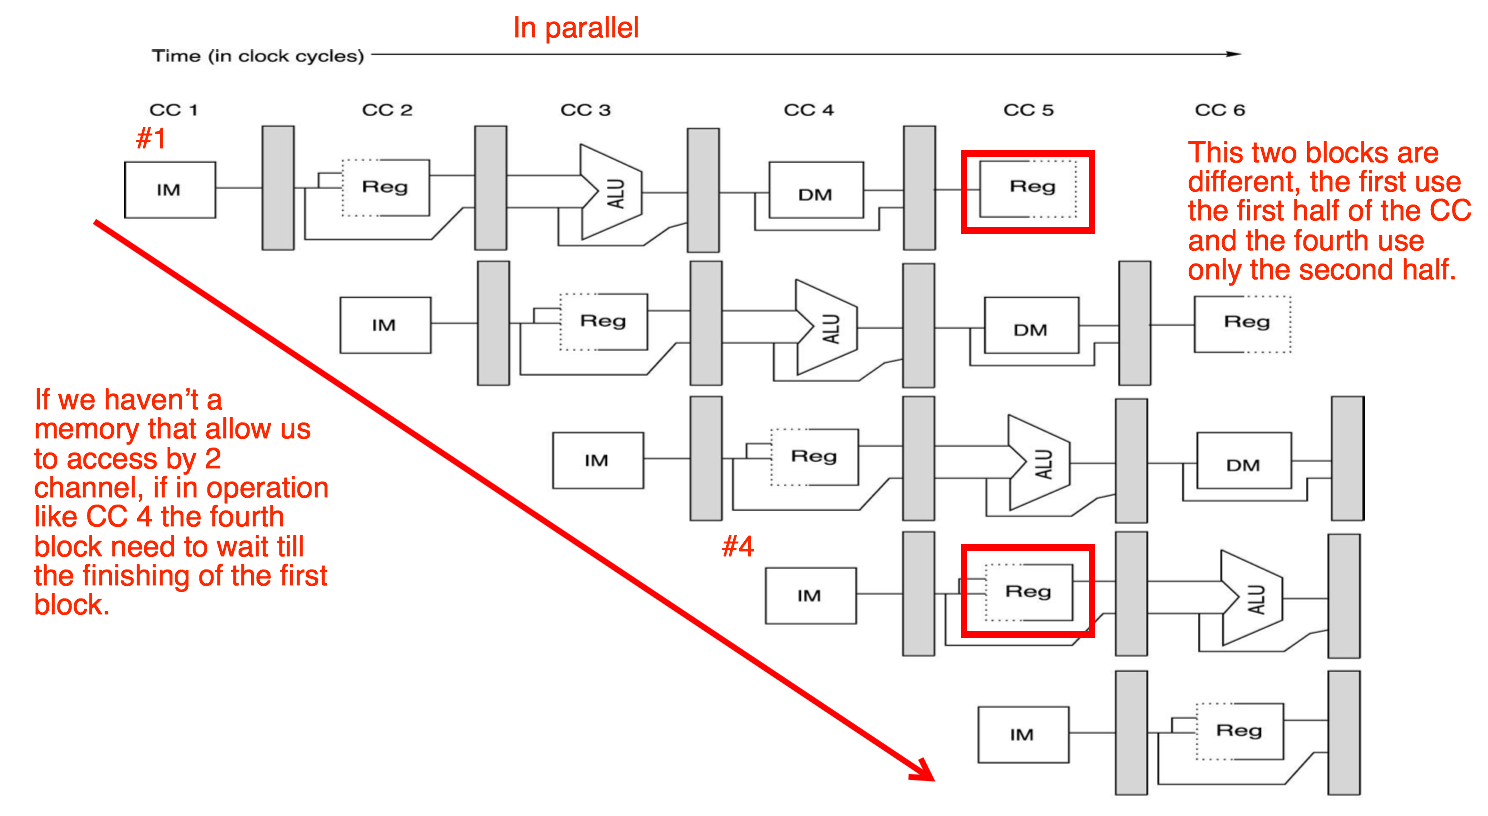
\includegraphics[width=\linewidth]{images/time_evo_pipe.png}
  \caption{Evolution in time of Pipeling architecture}
  \label{fig:time_evo_pipe}
\end{figure}

\paragraph{Performance} The first puorpose of this architectural type is the performance increase without making single instruction faster. The single instruction are maded slower for the overhead introduced by the pipeline control. The limitations of a pipeline come from the necessity of balanced stages and pipeling overhead (pipeline register delay and clock skew).

\subsection{Hazards}
The hazards are situations that prevent the execution of an instruction during its designated clock cycle. There are 3 classes of hazards:
\begin{itemize}
  \item \textbf{Structural}: Coming from resource conflict.
  \item \textbf{Data}: And instruction depends on the result of a previous instruction.
  \item \textbf{Control}:Depend on pipelining branches and other instructions that change the PC.
\end{itemize}
One way to dealing with hazards is to force the pipeline to stall, i.e., to block instructions for one or more clock cycles. When and instruction is stalled:
\begin{itemize}
  \item The instructions following the stalled instruction are also stalled.
  \item The instructions preceding the stalled instruction continue.
\end{itemize}
A stall causes the introduction of a bubble in the pipeline.

\paragraph{Structural hazards} they may happen when some pipeline unit is not able to execute all the operations scheduled for a given cycle. Example:
\begin{itemize}
  \item A given unit is not able to complete its task in one clock cycle (division).
  \item The pipeline owns only one register-file write port, but there are cycles in which two register writes are required.
  \item The pipeline refers to a single-port memory, and there are cycles in which different instructions would like to access to the memory target.
\end{itemize}
Solving this problem implies adding or improving the hardware.

\paragraph{Data hazards} overlapping the execution of instructions, as it is done by pipelining, changes the order of read/write accesses to operands. This can lead to wrong results and undeterministic behavior.\\
An example could be:\\
\begin{lstlisting}
ADD R1, R2, R3
SUB R4, R1, R5
AND R6, R1, R7
\end{lstlisting}
The second instruction will read the value of R1 before the first instruction can write the new value. This will cause a wrong result. And is the same of course for the third instruction.\\
If an \textbf{Interrupt effects} occurs during the execution of a critical piece of code (from the pov of data hazards) correctness may be restored. This may causa an undeterministic behavior.\\
There are two possibile solution for data hazards problems:
\begin{itemize}
  \item The first is using the stall till the data will be available.
  \item Implementing the \textbf{forwarding} technique.
\end{itemize}

\paragraph{Forwarding} A special hardware in the datapath detects when a previous ALU operation should write the register corresponding to the source of the current ALU. In this case, the hardware, selects the ALU result as the ALU input rather than the value from the register file. This part must be able to:
\begin{itemize}
  \item Forward a data from any of the previously started instructions (the data can't be already writed in its final location).
  \item Not to forward anything, if the following instruction is stalled, or an interrupt occurred.
\end{itemize}
an example can be viewed in the figure \ref{fig:forward_ex}.

\begin{figure}[h!]
  \centering
  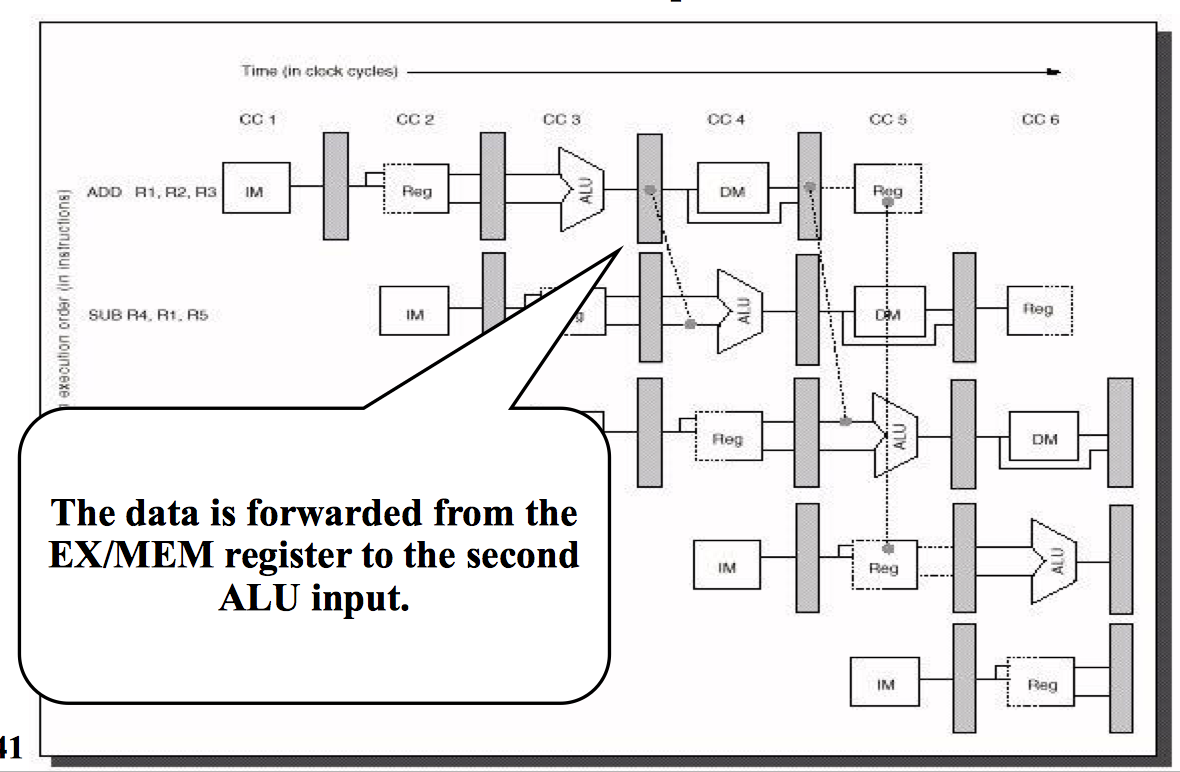
\includegraphics[width=\linewidth]{images/forward_ex.png}
  \caption{Forwarding Example}
  \label{fig:forward_ex}
\end{figure}

The forwarding can be implemented:
\begin{itemize}
  \item From the ALU or data memory output...
  \item ...to ALU inputs, data memory inputs, or the zero detection unit (branch instruction).
\end{itemize}
and the logic must compare:
\begin{itemize}
  \item The DEST fields of the IR in the EX-MEM and MEM-WB register with...
  \item ... the SRC fileds of the IR in the IF-ID, ID-EX and EX-MEM registers.
\end{itemize}

\paragraph{Causes of Data Hazards} A hazards is created whenever there is dependence betweem instructions, and they are close enough that the overlap caused by pipeling would change the order of access to an operand.
In general, this can happen for:
\begin{itemize}
  \item Register Operands
  \item Memory Operands:
  \begin{itemize}
    \item Acceses to memory by load and store are not made in the same stage.
    \item execution can proceed while an instruction waits for a cache miss to be solved.
  \end{itemize}
\end{itemize}
The forwarding not solve all potential data hazards, in this case to only solution is to use stalls.

\paragraph{Stalls} At each clock cycle all test for detecting data hazards are performed (ID stage), if an hazard is detected two actions can be taken:
\begin{itemize}
  \item The apporpriate forwarding is enabled.
  \item The instruction is stalled before entering in the wrong stage.
\end{itemize}
This situation can be performed in two ways:
\begin{itemize}
  \item Forcing all 0s in the ID-EX pipeline register (\textit{nop} instruction).
  \item Forcing the IF-ID pipeline register to maintain the current value.
\end{itemize}

\paragraph{Control Hazards} are due to branches, which may change the PC after the following instruction has been fetched already. In the case of conditional branches, the decision on whether the PC should be modified or not can be taken even later. In the MIPS implementation, the PC is written with the target address (if the jumo is taken) at the end of the ID stage.\\
A possible solution is based on stalling the pipeline as soon as a branch instruction is detected (ID stage) by:
\begin{itemize}
  \item Decide earlier whether the branch has to be taken or not.
  \item Compute earlier the new PC.
\end{itemize}

\paragraph{Performance} there are several techniques for reducing the performance degradation due to branches:
\begin{itemize}
  \item \textbf{Freezing pipeline}: the pipe is stalled until the decision about the branch is know.
  \item \textbf{Predict untaken}: Assume the branch is not taken, avoid any change in the pipe, undo all performed if the branch is taken. *
  \item \textbf{Predict taken}: If the target address is know before the branch outcome, it may be possible to assume the branch as taken. *
  \item \textbf{Delayes branch}: Filling the slot after the branch instruction (branch-delay slot) with instructions which have to be executed no matter the branch outcome. Is a compiler task. Less used nowadays.
\end{itemize}
* This thecniques can be speeded by the compiler which maximizes the chance for the processor to make the right prediction.\\

\subsection{Exception}
The execption are fundamental for system. The are a lot of possible causes:
\begin{multicols}{2}
  \begin{itemize}
    \item I/O device request
    \item System call by user program
    \item Tracing instruction execution (like debug mode)
    \item Breakpoint
    \item Overflow and underflow
    \item FP anomaly
    \item Page fault
    \item Misaligned memoery accesses
    \item Undifined instruction
    \item Hardware malfunction
    \item Power failure
  \end{itemize}
\end{multicols}
they can be calssified based on the type:
\begin{itemize}
  \item \textbf{Synchronous - Asynchronous}: Same position in code - External devices.
  \item \textbf{User requested - Coerced}: Like procedures - Out of user control.
  \item \textbf{User maskable - Non maskable}: Force hardware not to answer to exception requests.
  \item \textbf{Within - Between instructions}: Generated by instruction itself.
  \item \textbf{Resume - Terminate}: Terminate or execute something than resume.
\end{itemize}

There are some machine, called restatable, the are able to handle an exception, save the state, and restart without affecting the execution of the program. Nowadays all processors are restatable.\\

\paragraph{Stopping execution} when and exception occurs, the pipeline must execute the following steps:
\begin{itemize}
  \item Force a trap instruction into the pipeline on the next IF stage.
  \item Until the trap is taken, turn off all writes for the instruction that raised the execption and for all the following instructions in the pipeline.
  \item When the exception-handling procedure receives control, it immediately saves the PC of the faulting instruction.
\end{itemize}
after the exception has been handled, special instructions return the machine from the exception by reloading the PC and restarting the instruction stream.\\
A processor has precise execeptions if the pipeline can be stopped so that:
\begin{itemize}
  \item The instructions just before the faulting instruction are completed.
  \item The instructions following the faulting instruction ca be restarted from scratch.
\end{itemize}
It could be really hard restarting after exception, but precise execption is a must for most architectures, at least for integer.

\paragraph{Contemporary exception} for example we can have 2 different instruction LD that thrown an exeception during the MEM phase and a DADD that can generated an arthmetic exception during the EX phase. The handling could manage the first problem, and if its cause is removed, the second occurs. The situation can be different supposing that the DADD generate an error in the IF stage and the LD still in the MEM phase, this case generate before the DADD exception and then the other.\\
The are multiple solution, a good one could be:
\begin{itemize}
  \item A status flag is associated to each instruction in the pipeline.
  \item If an instruction causes an exception, the status flag is set.
  \item If the status flag is set, the instruction can not perform any write operation.
  \item When an instruction reaches the last stage, and its status flag is set, an exception is triggered.
\end{itemize}
In some cases machines have instructions that change the state before they are committed (those using autoincrement addressing modes). If one of these instructions is aborted because of an exception, it leaves the machine state altered. Implementig precise exceptions could be really tough.\\
Instructions implicitly updating condition codes create complications:
\begin{itemize}
  \item Data Hazards
  \item Save and restored in case of exception.
  \item Hardening the compiler work to filling delay slots between writing conditions and branch.
\end{itemize}

\subsection{Multicycle Operations}
Floating points units perform more complex operations than the integer ones. Forcing them to be executed in a single CLK means using a very slow clock or using really complex unit. The main solution is repeating the EX stage as many times as the instruction requires. An example for undestan the number can be viewed in this table below:

\begin{center}
  \begin{tabular}{ |c||c|c| }
    \hline
    \textbf{Functional Unit} & Latency & Init Interval\\
    \hline
    \textbf{Integer ALU} & 0 & 1\\
    \hline
    \textbf{Data Memory} & 1 & 1\\
    \hline
    \textbf{FP Add} & 3 & 1\\
    \hline
    \textbf{FP/Int Multiply} & 6 & 1\\
    \hline
    \textbf{FP/Int Divide} & 24 & 25\\
    \hline
  \end{tabular}
\end{center}
\textbf{Latency}: It is the number of cycles that should last between an instruction that produces a result and an instruction that uses the same result.\\
\textbf{Initiation Interval}: It is the number of cycles that must elapse between issuing two operations of the same type to the same unit.\\

\paragraph{Hazards} can be more frequent due to the different structure of the EX stage. This because:
\begin{itemize}
  \item Unpipelined divide unit, where several instructions could need it at the same time.
  \item The instructions have varying running times, the number of the register writes required in a cycle can be larger that 1.
\end{itemize}
solving this problem with more writes ports is normally too expensive, the solution is forcing a structural hazard stalling the instructions in the ID stage, or stalling it before the MEM or WB stage. This kind of operations can introduce long period of stall. This introduce new type of hazards, like \textbf{RAW} (Read After Write), \textbf{WAW} (Write After Write) and  structural hazards involving the divide unit and the write port.\\
A solution could be that, before issuing an instruction to the EX phase, check whether it is going to write on the same register of an instruction still in the EX stage. In this case, stall the new instruction. Of course guarantee the precise exception become really hard, the possible solutions are:
\begin{itemize}
  \item Accepting imprecise execeptions.
  \item Fast, but imprecise operating mode, and slow, but precise one.
  \item Buffering the results of each instruction until all the previously issued instructions have been completed.
  \item Forcing the FP units to early determine whether an instruction can cause an exception, and issuing further instructions only when the previous ones are guaranteed not to cause an exception.
\end{itemize}
An alternative solution is like the MIPS R4000 that implements a 8 cycle pipelined processors. This means more forwarding, increased load delay slot and increased branch delay slot.

\subsection{Instruction Level Parallelism}
The pipelines exploit the parallelism existing among instructions, which allows their execution in parallel. The highest the amount of ILP that can be found, the better the performance of the pipeline. There are two kind of approach:
\begin{itemize}
  \item Static: Depending on the software (i.e compiler). Used in embedded system.
  \item Dynamic: depending on the hardware to locate parallelism. Used in desktop and server.
\end{itemize}

The basic block is the group of instructions belonging to the same block, it means no branches in (except entry) and no branches out (excepts exit). The basic block is opmizable by the compiler by a little rescheduling. For example if we need to compute $a=b+c\\d+e-f$ on solution could be the one in figure \ref{fig:stall}:
\begin{figure}[h!]
  \centering
  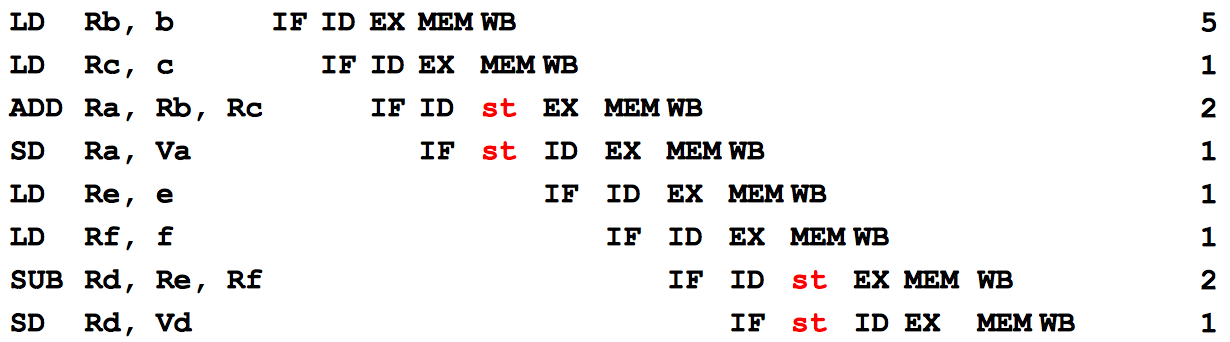
\includegraphics[width=\linewidth]{images/stall.png}
  \caption{First execution order}
  \label{fig:stall}
\end{figure}
that requires 14 clocks cycles. In figure \ref{fig:stall2} a better solution is implemented, this rescheduling requires only 12 clock cycles.
\begin{figure}[h!]
  \centering
  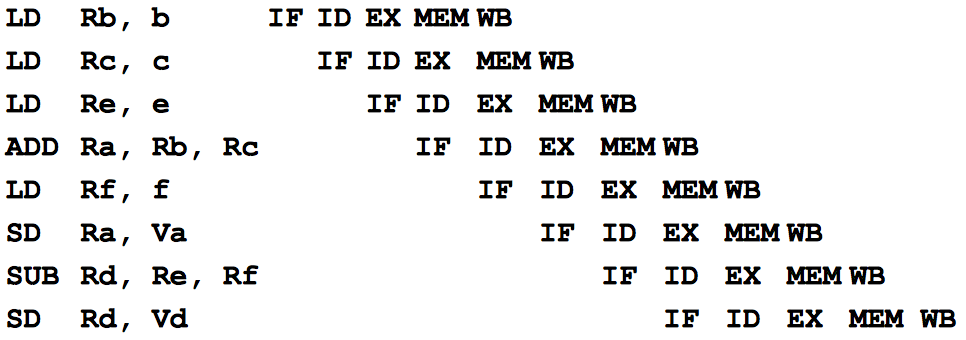
\includegraphics[width=\linewidth]{images/stall2.png}
  \caption{Second execution order}
  \label{fig:stall2}
\end{figure}
 For typical MIPS program the size of a basic block is between 4 and 7 instructions. Since these instructions are likely to be dependent one from the other, the amount of parallelism existing within a basic block is normally rather small.\\
 COnsidering a loop any iteration of a loop could be independent on the others, so they can be overlapped. There are two ways for exploting the loop-level parallelism:
 \begin{itemize}
   \item Loop unrolling (static or dinamyc)
   \item SIMD
 \end{itemize}

The first solution explicitly replicate the loop body in multiple times like in figure \ref{fig:unrolling}.
\begin{figure}[h!]
  \centering
  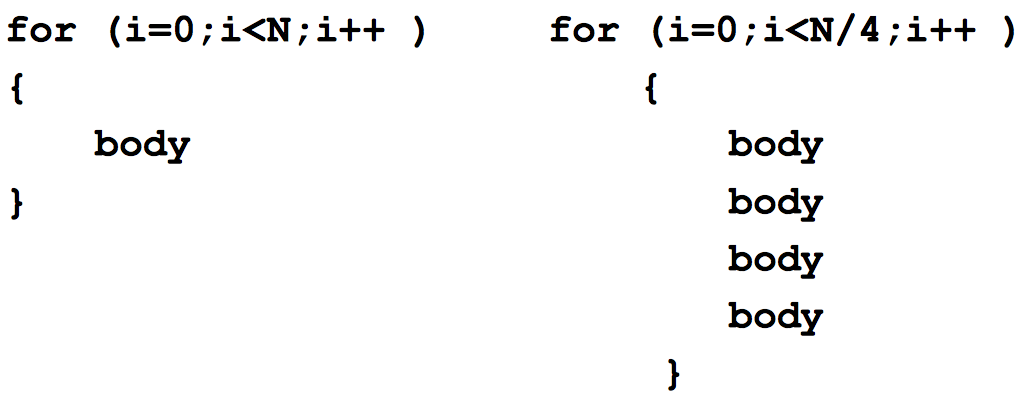
\includegraphics[width=\linewidth]{images/unrolling.png}
  \caption{Loop unrolling}
  \label{fig:unrolling}
\end{figure}
The considerations are:
\begin{itemize}
  \item[\textbf{+}] Reduced overhead due to the iteration control.
  \item[\textbf{+}] Wider body increase the chance for the compiler to exploit rescheduling to eliminate stalls.
  \item[\textbf{-}] Size code increased.
\end{itemize}

The SIMD techniques it can be exploited in:
\begin{itemize}
  \item Vector processors: A vector instruction operates on a set of data, instead of on a scalar data (as normal instructions).
  \item GPUs: Parallel acting over multiple data.
\end{itemize}

In both cases is necessary to evaluate the dependencies, if two instructions are not dependent, they can be executes in parallel without any stall. If they are not, they have yo be executed in order (or partly overlapped). There are 3 kind of dependencies: data, name and control.\\
An instruction \textit{i} is \textbf{DATA} dependent on instruction \textit{j}, if \textit{i} produces a result that is used by instruction \textit{j}, or if j is dependent on instruction \textit{k}, and \textit{k} is dependent on instruction \textit{i}.\\
Detecting dependencies involving registers is easy. Detecting dependencies involving memory cells is much more difficult, because accesses to the same cell can look very different. Using a static techniques force the compiler to adopt a conservative approch, assuming that anu load instruction refers to the same cell of the previous store. This kind of dependencies can be only detected at the tun time, when the addresses are known.\\
A \textbf{NAME} dependencies occurs when two instructions refer to the same register or memory location (name) but there is no flow of data associated to the name. They can be of 2 types:
\begin{itemize}
  \item \textit{Antidependence}: Instruction j writes a register or memory location that instruction i reads, and instruction i is executed first.
  \item \textit{Output dependence}: Both instruction i and j write the same register or memory location.
\end{itemize}
The name dependencies do not prevent from reordering involved instructions, provided that we change the register used by one of the two instructions, it can be exploited by compiler (statically) or by the processor (dynamically). A similar method can be implemented to solve name dependencies involving memory locations. Finding possibile hazards require carefully analyzing the code, taking also into account the effects of branches.\\
Another kind of dependecies is the control one, it occurs when an intruction depends on a branch. An instruction that is control dependent on a branch cannot be moved before the branch (so that its execution is no more controlled by the branch). Altought, an instruction that is not control dependent on a branch cannot be moved after the branch (so that its execution become dependent on the branch). Preserving the control dependencies is a sufficient condition for preserving the program correctness. The reverse is not always true! The critical properties for program correctness are:
\begin{itemize}
  \item Exception behavior
  \item Data flow
\end{itemize}
Changing in the instruction order must not change how exception are raised. Anticipating the LD before the BEQZ in this piece of code:
\begin{lstlisting}
DADDU R2, R3, R4
BEQZ R2, L1
LD R1, 0(R2)

L1: ...
\end{lstlisting}
is not possible because LD can cause an exception, no matter whether the branch is taken or not.\\
The data flow is easy to be understand, changing the order of some operations can change the final result of the software running therefor is important to pay attention on that problem.

\subsection{Branch Prediction Techniques}
Branches can potentially impact seriously on the pipeline, a solution can be to predict how branches will behave. Also in this case the are two main solution:
\begin{itemize}
  \item Static Techniques: Handled by the compiler resorting to a preliminary analysis of the code.
  \item Dynamic Techniques: Implemented by the hardware based on the behavior of the code.
\end{itemize}
The \textbf{static} solution become useful when cobined with other static techniques, delayed branches and rescheduling to avoid data hazards.
Th compiler may predict branch behavior in different alternative ways:
\begin{itemize}
  \item Predict branches as taken.
  \item Predicting behavior depending on branch direction: Forward branch often untaken, Backward branches more often taken.
  \item Prediction based on earlier runs: Try to run a limited number of times, gather statistics and use it for prediction.
\end{itemize}

Using the dynamic technique, the hardware is in charge of prediction. Starting from the branch instruction address to active different prediction mechanisms. There are some difference between possibile prediction:
\begin{itemize}
  \item Branch History Table (1 and 2 bit schemes).
  \item 2-level prediction schemes (correlating predictors).
  \item Branch-target buffer.
\end{itemize}
The \textbf{BHT} is the simplest method. Is a small memory indexed by the lower portion of the address of the branch instruction, containing for each entry one or more bits recording whether the branch has been taken or not in the last execution.\\
\textbf{Two-bit prediction} schemes provide higher prediction capabilities. For every branch, two bits are mantained, and the prediction is changed only after missing twice. There is also the \textbf{n-bit} solution that us n bit for performing a similar behavior of the previous method. When the counter value is greater than one half of tis maximum value, the branch is predicted as taken, when it is lower it is predicted as not taken.\\
The correlating predictors is an approach (also called two-level predictors) base on exploting dependencies between the result of branches, where the the behavior of a branch is strongly dependent on the result of the previous ones. They use the behavior of the last \textit{m} branches to choose from $2^m$ branch predictors, each of which is a \textit{n}-bit predictor. The hardware implementation is very simple:
\begin{itemize}
  \item The history of the most recent \textit{m} branches is recorded in an m-bit shift register, where each bit records whether the branch was taken or not.
  \item The branch-prediction buffer is indexed using a concatenation of the low-order bits from the branch address with the \textit{m} low-order history bits.
\end{itemize}

Reducing the negative effects of control dependencies requires knowing as soon as possible:
\begin{itemize}
  \item Whether the branch has to be taken or not.
  \item The new value of the PC (if the branch is assumed to be taken).
\end{itemize}
The later issue is faced by introducing a \textbf{Branch-Target buffer} (or cache). Each entry of the BTB contains:
\begin{itemize}
  \item \textbf{Address} of the considered branch.
  \item \textbf{Target} value to be loaded in the PC.
\end{itemize}
Using the BTB, the PC is loaded with the new value at the end of the IF stage, i.e., even before the branch instruction is decoded. The flow of this solution in figure \ref{fig:btb}.\\
The BTB could be used cobined with other strategy, like branch history table, if a two-bit prediction is adopted.
\begin{figure}[H]
  \centering
  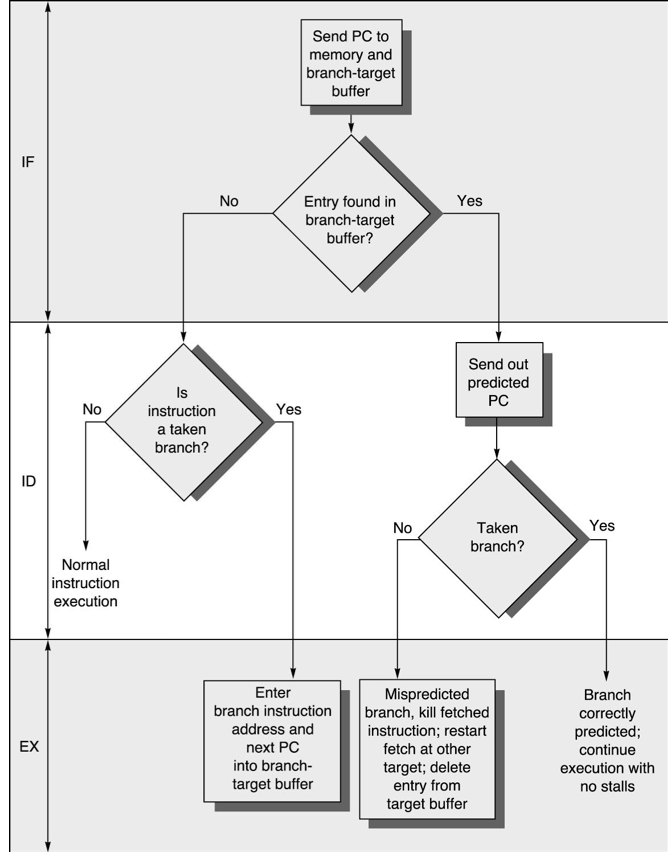
\includegraphics[scale=0.75]{images/btb.png}
  \caption{Branch-Target Buffer behavior}
  \label{fig:btb}
\end{figure}

\subsection{Dynamic Scheduling Techniques}
The \textit{dynamic scheduling} is a technique aimed at rearranging in hardware the instruction execution order to reduce the pipeline stalls while maintaining data flow and exception behavior. The advantages of DS are:
\begin{itemize}
  \item Identifies some dependencies that are unknow at compile time.
  \item Simplifies the compiler job.
  \item Allows the processor to tolerate unpredictable delays.
  \item Allows to run the same code on different pipelined processors.
\end{itemize}
Starting from this example:
\begin{lstlisting}
DIV.D F0, F2, F4
ADD.D F10, F0, F8
SUB.D F12, F8, F14
\end{lstlisting}
where the ADD instruction need to wait the end of the DIV for a data dependency, we can think about some DS solutions.\\
One possible solution for the proposed example is to remove the constraints of \textit{inorder instruction execution}. This implies some considerations, it may introduce:
\begin{itemize}
  \item WAR hazards
  \item WAW hazards
  \item Imprecise execeptions
\end{itemize}

If the out-of-order execution is allowed, precise exception handling is impossible. This may mean that at the time when the exception is raised:
\begin{itemize}
  \item An instruction before that raising the exception still has to be completed, or
  \item An instruction after that raising the exception has been already completed.
\end{itemize}
In both cases resuming program execution after exception handling becomes really difficult.\\
\textbf{Splitting ID stage} it useful to support out-of-order execution, it is splitted in two parts:
\begin{itemize}
  \item Issue: decode instruction, check for structural hazards.
  \item Read Operands: Wait until no data hazards, then read operands.
\end{itemize}
The issue stage reads instructions from a register or a queue (written by the IF stage). Instruction issue is performed in-order. After the instruction are issued, they may wait for operands, and then (when operands are available) sent to the EX stage. They can be stalled or bypass each other while in the read operand stage. Therefor, they can enter execution out-of-order.\\
If the processor includes multiple functional units, multiple isntructions may be in execution at the same time. Instructions can also bypass each other while in the execution stage. Therefor, they can leave execution out-of-order.\\
\paragraph{Hardware schemes} ont of the first solutions to achieve the dynamic scheduling was proposed in 1967 from an IBM architect, Robert Tomasulo. The key ideas in the Tomasulo's algorithm are:
\begin{itemize}
  \item Track the operands availability.
  \item Introduce register renaming.
\end{itemize}
The \textbf{reservation stations} are the key novelty in the Tomasulo's approch. They have several functions:
\begin{itemize}
  \item They buffer the operands of instructions waiting to issue; operands are stored in the station as soon as they are available.
  \item They implement the issue logic.
  \item The univocally identify and instruction in the pipeline: pending instruction designate the reservation station that will provide them with an input operand.
\end{itemize}
Using the register renaming allow to eliminate WAW and WAR hazards. Each time an instruction is issued, the register specifiers for the pending operands are renamed to the names of the reservation stations in charge of computing them. An example in figure:
\begin{figure}[h!]
  \centering
  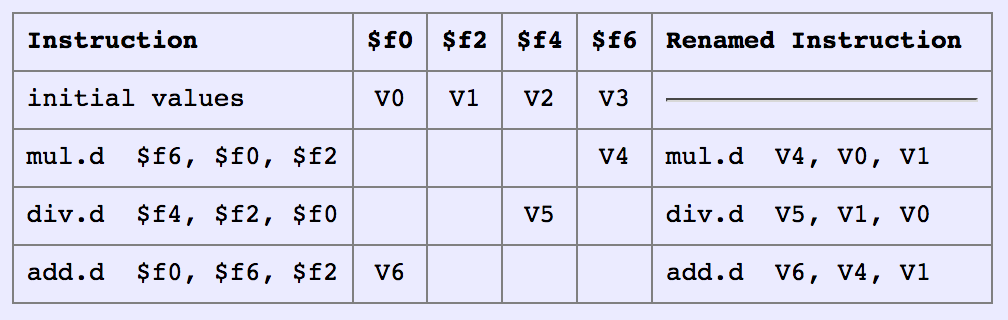
\includegraphics[width=0.7\linewidth]{images/rename.png}
  \caption{Register Renaming}
  \label{fig:rename}
\end{figure}
The reservation stations related to each functional unit control when an instruction can begin execution at that unit. Results are passed directly to other functional units, rather than going through the registers. All results from the functional units and from memory are sent to the \textit{Common Data Bus}, which:
\begin{itemize}
  \item Goes everywhere, execept to the load buffer.
  \item Allows all units waiting for an operand to load it simultaneously when it is available.
\end{itemize}

\paragraph{Issue} get an instruction from the instruction queue (implementing FIFO strategy):
\begin{itemize}
  \item If no reservation station is available, a structural hazard occurs, and the instruction stalls until a reservation station becomes available.
  \item If there is an empty reservation station, send the instruction to it:
  \begin{itemize}
    \item If the operands are available, they are sent to the reservation station.
    \item If not, the functional units responsible fo their generation are recorded.
  \end{itemize}
\end{itemize}

\paragraph{Flow} In case of normal instructions, when an operand appears on the CDB, it is read by the reservation unit. As soon as all the operands for an instruction are available in the RU, the instruction is executed. For the load and store operations, the first step is, as soon as the base register is available, the effective address is computed and written in the load/store buffer. The second step will be, for the load instruction: execute as soon as memory is available, for the store instructions, wait the operand to be written and then executed as soon as memory is available. In case of branches, to preserve exception Behavior, no instruction is allowed to initiate execution until all branches that precede the instruction in program order have completed. When the result of an instruction is available, it is immediately written on the CDB, and from there is the register and functional units waiting for it.\\

Each reservation station is associated with an \textbf{identifier}. It identify also the operand the instruction will produce. Instructions requiring that operand identify it using the identifier. The identifiers play the role of names of virtual registers that ca be used to implement register renaming.

\paragraph{RS Fields} the reservation station is divided in more field like in figure below:
\begin{figure}[H]
  \centering
  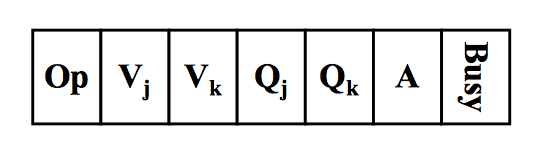
\includegraphics[width=0.6\linewidth]{images/rsf.png}
  \label{fig:rsf}
\end{figure}
where:
\begin{itemize}
  \item Op: Operation to be performed.
  \item $V_j, V_k$: Values of the source operands.
  \item $Q_j, Q_k$: Reservation stations that will produce a source operand.
  \item A: Used in l/s buffer only. Immediate field and then effective address.
  \item Busy: Status of the reservation station.
\end{itemize}

The \textbf{register file} contains, for each element, one field $Q_i$; that is the number of the reservation station that contains the instruction whose result should be stored in the register. If is \textit{null}, no currently active instructions computing a result destinated to this register.\\

In figure \ref{fig:ers} an example of the reservation station for this code:
\begin{lstlisting}
L.D F6, 34(R2)
L.D F2, 45(R3)
MUL.D F0, F2, F4
SUB.D F8, F2, F6
DIV.D F10, F0, F6
ADD.D F6, F8, F2
\end{lstlisting}
\begin{figure}[H]
  \centering
  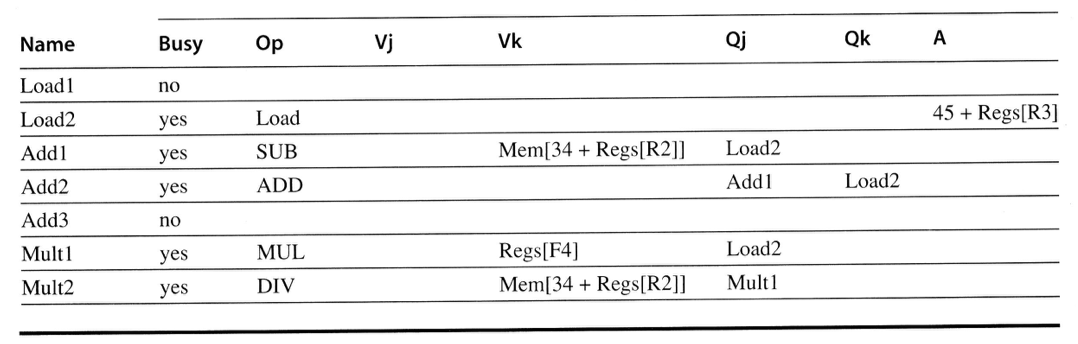
\includegraphics[width=\linewidth]{images/ers.png}
  \caption{Reservation station of the example}
  \label{fig:ers}
\end{figure}
The register file is represented in figure
\begin{figure}[H]
  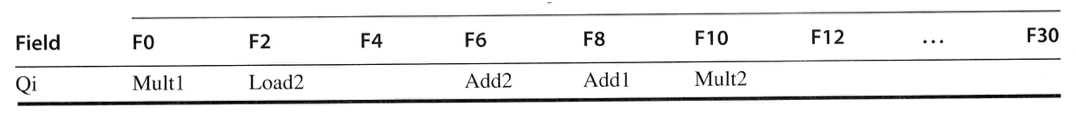
\includegraphics[width=\linewidth]{images/erf.png}
  \caption{Reservation station of the example}
  \label{fig:erf}
\end{figure}

There are several advantages using this solution:
\begin{itemize}
  \item The hazard detection logic is distruited.
  \item Stalls for WA and WAR hazards are elimnated.
  \item Loop unrolling not required, naturally performed in parallel.
\end{itemize}
there are also some disadvantage:
\begin{itemize}
  \item High complxity hardware (including an associative buffer for each RS).
  \item The CDB can be a bottleneck.
\end{itemize}

\subsection{Hardware-based Speculation}
The HBS is a technique for reducing the effects of control dependences in a processor implementing dynamic scheduling. If a processor supports branch prediction with DS, it \textit{fetches} and \textit{issues} instructions, as if the branch prediction was always correct. If a processor support BHS, it also \textit{executes} them.\\
The HBS combines three ideas:
\begin{itemize}
  \item Dynamic Branch Prediction
  \item Dynamic Scheduling
  \item Speculation
\end{itemize}
Is such way, the processor implements \textbf{data flow execution}: \textit{Operations execute as soon as their operands are available}.\\

\paragraph{Architecture} it implements the basic Tomasulo's architecture, extending it to support speculation.\\
There are two different steps in instruction execution:
\begin{itemize}
  \item The computation of results and their bypassing to other instructions.
  \item The update od register file and memory, which is only performed when the instruction is no longer speculative (instruction commit); in this way, in-order commitment is implemented.
\end{itemize}

Is introducce a new datastructure, the \textbf{ReOrder Buffer} (ROB), it contains the instruction results while the instruction didn't commit yet. It provides additional virtual registers and integrates the store buffer existing in the origianl Tomasulo's architecture.\\
In the TM's architecture already computed results are read from the register file. With speculation, data may be read:
\begin{itemize}
  \item from the ROB, if the producing instruction didn't commit yet.
  \item from the register file, otherwise.
\end{itemize}
Each entry of the ROB has four fields:
\begin{itemize}
  \item Instruction Type: Branch, store, or register.
  \item Destination: Register number, or memory address.
  \item Value: Contains the value when the instruction has completed but still didn't commit.
  \item Ready: Indicates whether the instruction completed its execution.
\end{itemize}

\paragraph{Steps} this solution provides four execution steps. The first is the \textbf{Issue} (or Dispatch) step:
\begin{enumerate}
  \item An instruction is extracted from the instruction queue id there is:
  \begin{itemize}
    \item an empty reservation station and
    \item an empty slot in the reorder buffer.
  \end{itemize}
  If this not the case, the instruction issue is stalled.
  \item The operands for the instruction are sent to the reservation station, if they are in the register file or in the reorder buffer.
  \item The number of the reorder buffer entry for the instruction is sent to the reservation station to tag the instruction (and its results, when they will be written on the CDB).
\end{enumerate}

The \textbf{execute} step flow is:
\begin{itemize}
  \item The instruction is executed as soon as all the required operands are available (Avoid RAW hazards).
  \item Operands are possibly taken from the CDB as soon as another instruction produces them.
\end{itemize}
The lenght of this step varies depending on the instruction type (e.g. 2 for load instructions, 1 for integer instruction and different values for FP instructions).

Another important step is the \textbf{Write Result}:
\begin{enumerate}
  \item A soon as it is available, the result is put on the CDB (together with the tag identifying the instr.) and sent to the ReOrder Buffer.
  \item Any RS waiting for the result reads it.
  \item The RS is marked as available.
\end{enumerate}

The last step is the \textbf{Commit} (or Completion) step:\\
The ReOrder Buffer is ordered according to instructions original order.\\
As soon as one instruction reached the head od the buffer:
\begin{itemize}
  \item If it is a mispredicted branch, the buffer is flished, and the execution is restarted with the correct successor of the instruction.
  \item Otherwise, the result is written in the register or in memory (in case of a store).
\end{itemize}
In both case the ROB, implemented as a \textit{circular buffer}, entry is marked as free.

Since a dynamic renaming is implemented and memory updating occurs in-oder WAW or WAR hazards can't occurs. RAW hazards instead are prevented by:
\begin{itemize}
  \item Enforcing the program order while computing the effective address of a load wrt all earlier store instruction, and
  \item not allowing a load to initiate its second step if any active ROB entry occupied by a store has a destination field matching the A field of the load.
\end{itemize}

Th \textbf{store} instructions write to memory when they commit, only. Therefor, their input operand is required when they commit, rather then in the WR stage. This means that the ROB should have a further field, specifying where the input operand for each store instruction should come from.\\
\textbf{Exceptions} are not executed as soon as they are raised, but they are stored in ROB. When the instruction is committed, the possible exception is executed, and the following instructions flushed from the buffer.If the instruction is flushed from the buffer, the exception is ignored. Full precise exception handling is thus supported.\\

When a time-expensive event (e.g. second-level cache miss, TLB miss) occurs speculatively, some processors wait for its execution until the event is no more speculative. On the other side, low-cost events (e.g. first-level cache miss) are nomally executed speculatively.

\section{Mutiple-issue Processors}
The techniques for reducing the effects of data and control dependencies can be further exploited to obtain a CPI less than one. The are two kinds of processors able to do so:
\begin{itemize}
  \item Superscalar, either statically or dinamically scheduling instruction.
  \item Very Long Instruction Word (VLIW).
\end{itemize}

\subsection{Scheduling}
\paragraph{Statical Scheduling} Implementing a superscalar processors able to possibly issue several instructions according to the static order defined by the compiler is rather easy and inexprensive. Two instructions can be issued per clock cycle if: one is a load, store, branch or integer ALU operation, and the other is any FP operation (but load and store, whihc belong to the first category).
Two instructions (64 bits) are fetched and decoded at every clock cycle. The two instruction are aligned and constritute an \textbf{issue} packet. In the previous version of superscalar a fixed structure for issueing is need, not they don't have this limitations.\\
At each clock cycle 2 instructions must be read from the instruction memory. If they belong to different cache blocks, several processors fetch one instruction only. In general the issue packet may only contain one branch.\\
In order to obtain a real benefit, the FP units should be either pipelined, or mutiple and independent. When the first instruction is a FP load, store, or move, there is a possible contention for a FP register port, the possible solutions are:
\begin{itemize}
  \item Forcing the 1th instruction to be executed by itself.
  \item Giving the FP register file an additional port.
\end{itemize}
Another common problem occurs when the second instructions read the result of the first one, in this case a RAW is also possible. The most used solution is to delay the second instruction of one clock.\\

In the MIPS pipeline, load has a latency of one clock cycle, which means that in the superscalar pipeline the result of a load instruction can not be used on the same clock cycle but on the next one. In the static version the load delay slot (as well as the branch delay slot) is equal to three. The static multiple-issue scheduling is manly adopted by processors for the embedded market, such as those by MIPS.

\paragraph{Dynamic Scheduling} It can be obtained by adopting a scheme similat to the Tomasulo one. TO make the implementation easier, instructions are never issued to the reservation stations out-of-order. Is some clock cycles, more than one isntruction may be ready to write on the CDB, that can only service one isntruction at a time. Duplicating the CDB can provide higher performance, at the cost of some area overhead.

\paragraph{VLIW} Super scalar processor evelution led to complex processors composed of several functional units, and all the logic for:
\begin{itemize}
  \item Detecting and managing dependencies.
  \item Dynamic Scheduling.
  \item Branch prediction and speculation.
\end{itemize}
This increased a lot the complexity of processors. Alternative approaches have also been investigated, including VLIWs.

This type of processors have longn isntructions encoding several operations, which are issued in parallel. The hardware includes as many functional units, as the operations in a single instruction. They are relatively common for embedded applications (signal processing and graphics).
The basic characteristics are:
\begin{itemize}
  \item \textbf{More Complex Software}: It is up to the compiler to decide ehich instructions to pack togheter, exploting parallelism, unrolling loops, scheduling code across basic bloxks, etc.
  \item \textbf{Simpler Hardware}: It does not perform any check on possible dependencies among instructions (left to compiler).
\end{itemize}
When an operation require stalling the whole instruction packet is stalled, in order ot preserve the flow decided by the compiler.\\
A VLIW processors does not require the hardware for choosing the instruction to be executed in parallel (i.e., for detecting depenedencies). This kind of processor is limited by:
\begin{itemize}
  \item Inherent limitations of ILP in programs: Hard to find sufficient number of independent instructions that can be executed in parallel.
  \item Difficulties in building the hardware: More units, more bandwidth to register file and the memory.
  \item Limitations specific to a superscalar or VLIW processor.
\end{itemize}
The code size is much larger for VLIW processors, mainly due to two factors:
\begin{itemize}
  \item Loops are intesively unrolled to extract more parallelism.
  \item The empty slots in instruction encoding.
\end{itemize}
Sometimes instructions are compressed in memory and expanded when loaded to the processor.\\
The main bottleneck is caused by the memory, since the required bandwidth is higher, and stall due to cache misses cause a stall on the whole processor.\\
Two example are Trimedia TM32 (NXP, 5 instruction, statical) and Transmeta Crusoe (2/4 instructions).

\section{Thread Level Parallelism}
\subsection{Introduction}
It is unlikely that further eveolutions in processor or compiler architecture could achieve singificant improvements in the explotation of the available ILP. On the other side, in many applications there is a significant amount of parallelism available at a higher level (TLP).\\
A \textit{thread} is a separete process with its own instructions and data. A thread may correspond to:
\begin{itemize}
  \item A process within a parallel porgam consisting of multiple processes, or...
  \item An independent process.
\end{itemize}
There are applications that naturally expose a high degree of tTLP (e.g., many server applications, OS). In other caes, the software is written in such a way to explicitly express the parallelism. In some existing applications it can be relatively difficult to identify and exploit TLP.

\subsection{Multithreading}
In principle, ILP and TLP can be combined: an ILP-oriented processor could use TLP as a source of independent instructions to feed the available functional units as much as possible.\\
Multithreading allows mutiple threads to share the functional units of a single processor in an overlapping fashion, duplicating only threads private state. It requires:
\begin{itemize}
  \item Independently storing the state of each thread (register file, PC, page table, etc.)
  \item Independet access to memory (e.g., through the virtual memory mechanism)
  \item Effective mechanism for switching ffrom one thread to another.
\end{itemize}
There are different types of multithreading:
\begin{itemize}
  \item Fine-grained: The switch from one thread to another happens at every clock cycle.
  \item Coarse-grained: The switch happens only when an expensive stall aries.
  \item Simultaneous (SMT): It mixes fine-grained and superscalar ideas.
\end{itemize}
In the \textbf{fine}-grained multithreading the execution of multiple threads is interleaved (e.g., in a round robin fashion, skipping any thread which is stalled at a given time). The CPU must be able to efficiently switch between tasks at any clock cycle. The ADVANTAGE is that when an instruction is stalled, other instructions can be found in other threads, avoiding any performance loss. The main DISADVANTAGE is that threads could be slowed down by the concurrent execution of other threads.\\
The \textbf{coarse}-grained multithreading switch to a new thread only on costly stalls, the ADVANTAGE is that thread switch can be less efficient and the DISADVANTAGE comes from the impossibility to avoid the losses from short stalls.\\
This last solutions \textbf{SMT} is a type of fine-grained multithreading enabling a superscalar processor to exploit ILP and multithreading at the same time. Multiple instructions from independent threads can be issued using dynamic scheduling capabilities to resolve dependencies among them. Instructions from multiple threads can be mixed in the data path thank to:
\begin{itemize}
  \item High number of available registers.
  \item Renaming mechanism.
\end{itemize}
The SMT can be implemented on the top of an out-of-order processor by:
\begin{itemize}
  \item Adding a per-thread renaming table.
  \item Keeping separate PCs.
  \item Allowing instructions from multiple threads to commit (separate ROB from each threads).
\end{itemize}

\subsection{Conclusions}
Nowadays the trend is not towards embedding SMT in aggressive speculative processors.\\
Rather, designers are opting to implement multiple CPU cores on a single die with less aggressive support for multiple issue and multithreading.

\section{Cache memories}
\subsection{Introduction}
Cache memories are small and high-speed memories that are interposed between the processor and the main memory.\\
The presence of a cache can improve the performance of a system due to the \textbf{locality of referneces} observed in most programs. Locality takes two forms:
\begin{itemize}
  \item \textbf{Temporal}: If a time \textit{t} the program accesses to a given memory call, it is highly probable that the program accesses again the same cell by the time $t_0 + \delta t$.
  \item \textbf{Spatial}: If at time $t_0$ the program accesses a memory cell with addess X, it is highly likely that by the time $t_0 + \delta t$ the program will also access the memory cell with address X $\pm$ e.
\end{itemize}
The idea is that, at the time $t_0$ an entire block is loaded in the cache, it is likely that for a certain time $\delta t$ the program will find in the cache all of the words it needs.

\subsection{Organization \& Behavior}
A cache is organized in lines, each lines contains a memory block that includes some memory words. They are also associated with a tag field, which indicates the memory block present in that line at that time. The cache also contains the logic for:
\begin{itemize}
  \item Intercepting the addresses procuded by the processor.
  \item Checking inside the cache the possible presence of the block that the processor wants to access.
  \item Possibly loading the block.
\end{itemize}
\begin{figure}[h!]
  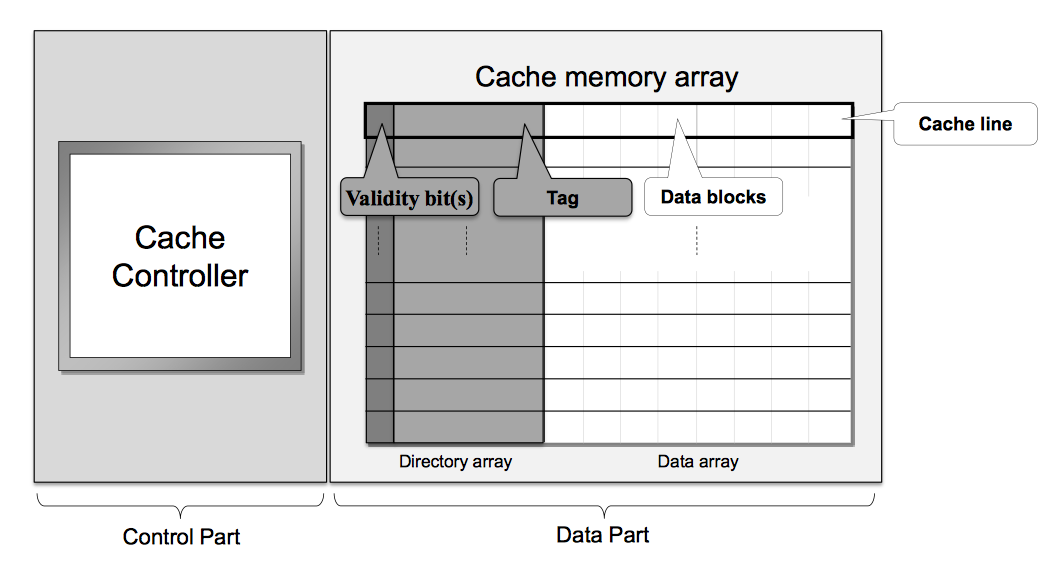
\includegraphics[width=\linewidth]{images/cacheOrg.png}
  \caption{Cache organization schems}
  \label{fig:cacheOrg}
\end{figure}

The cache is locate between the processor and the main memory. Each time the processor performs an access to memory the cache intercepts the address and check if the block to which the word belongs is in the cache, checking the value of the tags.
\begin{itemize}
  \item \textbf{if YES}: It extracs the word from the block and provides it to the CPU without any access to the main memory (CACHE HIT).
  \item \textbf{if NO}: It loads in the cache the entire block that the word is part of (CACHE MISS).
\end{itemize}
In case of a hit, the cache reducces the memory access times by the factor that is dependent on the ration between cache and primary memory access times.\\
In case of a miss, the cache responds in two possible ways:
\begin{itemize}
  \item It accesses the memory and loads the entire missing block; the it provides the requestd word. The access time is therefor higher that in a cache-free system.
  \item It accesses the memory and immediatly provides the requested word (load-through or early restart). This technique requires a higher cost in terms of cache hardware, but miss situations have more limited impact on cache performance.
\end{itemize}
Postitioning the cache between the CPU and the bus allows to gain some benefits reduce the bus load and compatible solution with multiprocessor architecture.

\subsection{Architecture}
If there are two caches, the architecture of the system falls into the scheme know ad Harvard architecture, characterized by the existence of two separate data and code memories. Important parameters of a cache memories are:
\begin{itemize}
  \item Cache size
  \item Mapping
  \item Replacing algorithm
  \item Main memory update mechanism
  \item Block Size
\end{itemize}
The \textbf{size} is very important, a size increase implies cost and system performance increase, but it becomes slower itself. The \textbf{mapping} mechanism defines in which line of the cache a certain memory block is written when it is uploaded in the cache. You must endure (at an accptable cost) that the cache can quickly verify if it contains the data corresponding to a certain address.
\begin{figure}[h!]
  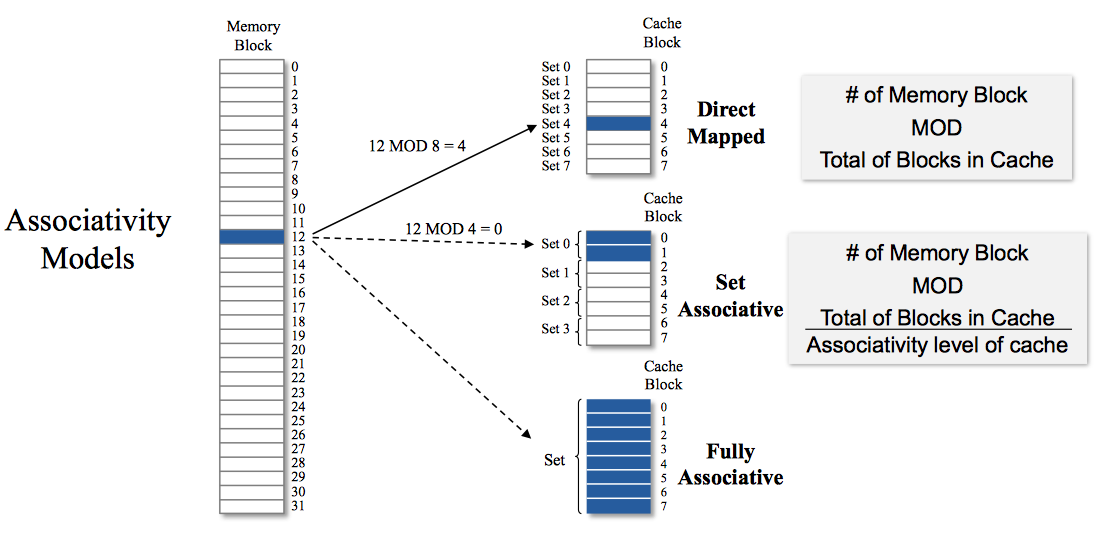
\includegraphics[width=\linewidth]{images/mapping.png}
  \caption{Mapping schemes}
  \label{fig:mapping}
\end{figure}
There are three main types of mapping. In the \textbf{Direct} mapping each memory block \textit{i} is statically associate to a line \textit{k} in the cache using the expression:
\begin{equation}
  \begin{gathered}
    k = i mod(N)
  \end{gathered}
\end{equation}
where N is the number of lines in the cache. The computation of \textit{k} can be easily performed by just taking the least significant bits in the i value. The advantage is that the mechanisms can be easily implemented in hardware, the problem is the if the program frequently accesses 2 blocks corresponding to the same cache line, a miss occurs at each momory access.\\
The \textbf{Set Associative} mapping divides the cache lines in \textit{S} sets, each consisting of \textit{W} (ways: 2 or 4 normally) lines, a block \textit{i} is associated with the set \textit{k} with $k = i mod(S)$, then the block \textit{i} can be put into any of the \textit{W} lines of the set k. This technique is also called \textit{W-ways} cache.\\
The last technique is the \textbf{Associative} mapping, each block of the main memory can be stored in any cache block. The main advantage is that there is maximum flexibility in choosing the cache block to use. The problem is complexity of search hardware.

\subsection{Replacing algorithm}
It defines which cache line should be used to store a memory block, amongest those associated with the block (in the case of associative or set associative mapping). The choice is over:
\begin{itemize}
  \item \textbf{LRU} (Least Recently Used): Most used.
  \item \textbf{FIFO} (First In First Out): Cheapest.
  \item \textbf{LFU} (Least Frequently Used): Theoretically, the most effective.
  \item \textbf{Random}: Simple and effective.
\end{itemize}

\subsection{Memory update}
When a write operation is performed on a data in the cache, we also need to update the main memory, there are two solutions that can be adopted. In the \textbf{Write-Back} for each cache block, a flag (called dirty-bit) is introduced, which remembers wheter ot not the block has been changed since it was loaded into the cache. When a block is evicted from the cache and the dirty bit is set, the block is copied from the cache to the main memory. Disadvantages:
\begin{itemize}
  \item The replacement is slower because it sometimes requires copying in the main memory the replaced block.
  \item In multiprocessor systems there may be incoherence between the caches of different processors.
  \item It may noy be possible to restore memory data after possible system failures.
\end{itemize}
The \textbf{Write-Through} solution instead, each time the CPU performs a write operation, it writes on both the cache data and the main memory data. The resulting loss of efficency is limited by the fact that writing operations are usually much less numerous that reading ones.

\subsection{Cache Coherence}
The cache coherence is the major problem in multiprocessor systems with shared memory, in which each processor has its own cache. Similar problems may occur if the system uses a DMA controller.\\
To achieve coherence, a vilidity bit is introduced for every cache line. If it is disabled, it means that any access to the block must produce a miss. At the power-on, the validity bits of all cache lines are disabled.

\subsection{Levels}
Modern arechitectures implements multiple-levels architectures, the L1 is the fastest but smallest ones, the L3 is the biggest but the slowest and the L2 is in the middle. Each time the processor performs a memory access:
\begin{itemize}
  \item It checks first whether the word is in L1.
  \begin{itemize}
    \item If so, it can access the world in L1.
    \item If not, it checks wheter the word is in L2.
    \begin{itemize}
      \item If so, it will access to the word in L2 and eventually update L1.
      \item If not, it checks wheter the word is in L3.
      \begin{itemize}
        \item If yes, L3 is accessed and L2 is updated.
        \item If not, it access to the main memory and eventually update L3.
      \end{itemize}
    \end{itemize}
  \end{itemize}
\end{itemize}
\begin{figure}[h!]
  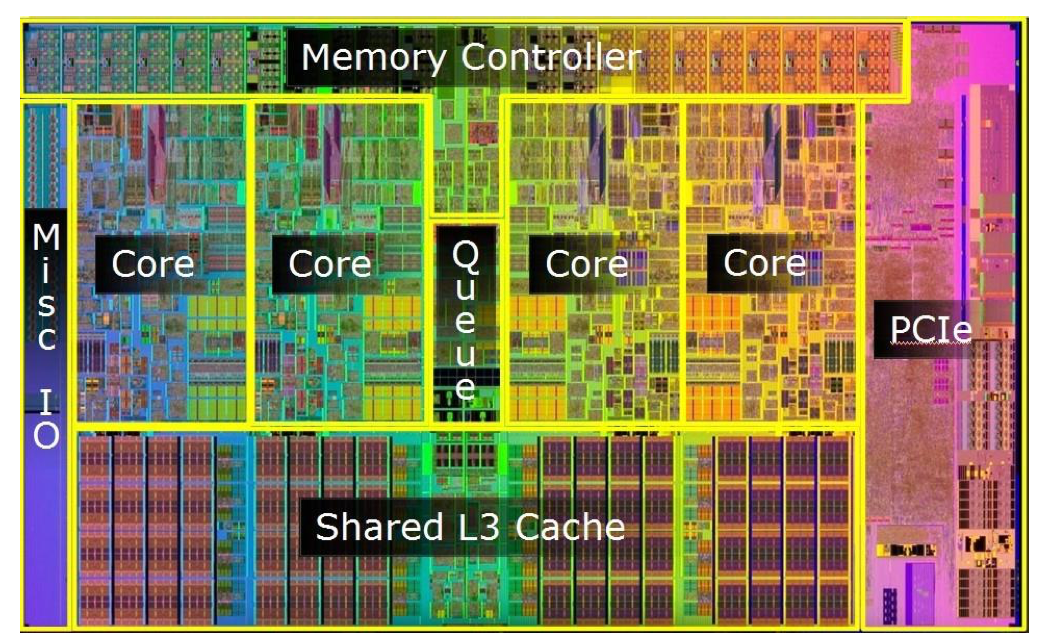
\includegraphics[width=\linewidth]{images/intel.png}
  \caption{Modern CPU schemes}
  \label{fig:intel}
\end{figure}

\end{document}
